\documentclass{hertieteaching}
\usepackage{cancel}
\usepackage{hyperref}

\title{words in space}

\begin{document}

\maketitle

\begin{frame}{the space of words}

we have seen a lot of \textit{document} spaces:
\begin{itemize}
  \item Rows in a \textit{document feature matrix} as coordinates in a $V$ space
  \item Word frequency distributions, e.g. DFM rows normalized to 1, as coordinates in a ($V$-1) dimensional simplex 
  \item Topic counts as locations in a $K$-dimensional space
  \item Topic proportions as location on a the corresponding $K$-1 dimensional simplex
\end{itemize}
Later, with scaling, we'll put documents into much smaller spaces, e.g. one or two dimensions.

But what about the words?
\begin{itemize}
  \item Do they live in a space?
\end{itemize}

\end{frame}

\begin{frame}{distributional hypothesis}

Back in the mid-20th century \textit{description} and \textit{empirical data gathering} hit linguistics, arguably from \textcite[]{Zipf1932} but also from field linguistics \parencite{Harris1954}.

Eventually this developed into \textit{distributional semantics} \parencite[e.g.][]{Cruse1986,}, which can be summarised informally as

\bigskip
\begin{quote}
You shall know a word by the company it keeps \\
\hfill\parencite{Firth1968}
\end{quote}

This is the linguistics counterpart of \textcite{Quine1960} or Wittgenstein's (\citeyear{Wittgenstein1958}) advice: Don't look for the meaning, look for the use.

Operationally:
\begin{itemize}
  \item The meaning of a word is the sum total of all the ways it is used in actually existing language
\end{itemize}

\end{frame}

\begin{frame}[fragile]{characterizing use}

A common test of language understanding: the sentence completion test. Fill in the missing word

\small
\begin{verbatim}
           All I want is a nice [       ] of tea
\end{verbatim}
\normalsize
  
A common descriptive tool for word usage: the keyword in context

\begin{center}
\small
\begin{verbatim}
      that "the state shall not [discriminate] against, or grant preferential treatment
the lingering effects of racial [discrimination] against minority groups in this
 remedy the effects of societal [discrimination]. Another four Justices (Stevens
      that "the state shall not [discriminate] against, or grant preferential treatment
\end{verbatim}
\normalsize

\end{center}

 These are closely alternates:
 \begin{itemize}
  \item By studying enough keywords in context you can learn to complete sentences
  \item Words mean the same to the extent you can substitute them into the same contexts, c.f. `bias'
\end{itemize}

  
\end{frame}

\begin{frame}[fragile]{Context vectors}

One simple way to characterize all those lines of kwic is to just \text{sum them up} 

A context-feature matrix $C$ where $C_{ij}$ is the number of times word $j$ occurred in word $i$'s kwics

Rows of $C$ are `context vectors' (Naturally, this depends on the window size)

Intuition: if two words are easily \textit{intersubstitutable in context} then 
\begin{itemize}
  \item their contexts share a lot of words
  \item so their context vectors should be similar
\end{itemize}

Geometrically
\begin{itemize}
  \item Context vectors should point in the same direction
  \item The angle between them should be small
  \item the cosine of that angle should be positive 
\end{itemize}

\end{frame}
\begin{frame}[fragile]{Caveats}

But wait, you say. What if there is more than one sense of word $i$? e.g. `bank' in English.
\begin{itemize}
  \item Mostly we just ignore it (and it's mostly fine\ldots)
\end{itemize}
Unlike the unimportance of negation, I'm not so sure I have a good explanation for this
\begin{itemize}
  \item Senses do seem to be roughly power law distributed \parencite{Zipf1945}, so maybe we just don't often need the infrequent ones for evaluation tasks?
\end{itemize}

\pause

Some people think there are reasonable senses of similarity that are \textit{asymmetric}

\smallskip
\begin{quote}
``No, Danish is not similar to German, German is similar to Danish''\\
\hfill (Unknown Danish nationalist, circa 1998)
\end{quote}

We shall quietly ignore the non-symmetric senses of similarity because their `distances' won't obey the triangle inequality.


\end{frame}


\begin{frame}[fragile]{semantic space}

Or as they call it these days: \textit{word embedding}

Four approaches:
\begin{itemize}
  \item Just use $C$, possibly with transformed elements \parencite{Bullinaria.Levy2012}
  \item Matrix factorizations of $C$, e.g. latent semantic indexing \parencite[LSI;][]{Landauer.Dumais1997} or \textsf{GloVe} \parencite{Pennington.etal2014}
  \item Some intermediate representation extracted from a neural network, e.g. \textsf{word2vec} \parencite{Mikolov.etal2013}, though it's not so clear that the \textit{neural network} part is doing the work
\end{itemize}

Let's dig into these after considering the kind of association we need\ldots

\end{frame}
\begin{frame}{Associations}

The key distributional semantics concept \textit{intersubstitutability in context} is a \textit{second order} similarity / association

\medskip

\textsc{First order similarity/ direct association}

`racial' and `discrimination' are associated when they tend to occur together, e.g.
\begin{itemize}
  \item as measured by a \textit{collocation} measure
\end{itemize}

\pause

\textsc{Second order association}

`bias' and `discrimination' as associated because they have similar associations with `racial'
\begin{itemize}
  \item two words are similar when they have the same \textit{pattern of first order associations} with all the other words in the vocabulary
\end{itemize}

\end{frame}

\begin{frame}{Associations}

In simple context feature matrix, $C_{ij}$ (how many times $j$ occurred in $i$'s contexts) is enough. 
\begin{itemize}
  \item Maybe (as in LSI) we shrink $C$ by Singular Value Decomposition
\end{itemize}

In fancier models, $C_{ij}$ is replaced by a `chance corrected' transformation like `pointwise mutual information'

In a (unrealistic) one token window:
$$
\text{PMI} = \frac{P(\text{racial}_n\text{ discrimination}_{n+1})}
{P(\text{racial}) P(\text{discrimination})}
$$ 

Note that by removing $P(\text{racial})$ from this we get an estimate of $P(\text{racial} \mid \text{discrimination})$


\end{frame}
\begin{frame}{Associations}

\textsf{GloVe} \parencite{Pennington.etal2014} is a little more sophisticated and assumes that it is \textit{relative usage} that drives association
$$
\text{log}~\frac{P(\text{racial} \mid \text{discrimination})}
{P(\text{racial} \mid \text{bias})}
$$
but in a \textit{proportional} way, so we log it (is this starting to seem familiar?)

\pause

Although \textsf{GloVe} would not describe it this way we can think of it as choosing context vectors $\beta_i, \beta_j$ to model the odds ratios underlying $C$
$$
\text{log}~C_{ij} = a_i + b_j + \beta_i \beta_j
$$
This is the reduced form of a log bilinear model of $C$ (but fit with weighted least squares)

If we choose a $K<V$-dimensional space then we are claiming that facts about relative usage are less 
variable than the words

\end{frame}


\begin{frame}[fragile]{Vector similarity}

OK, so we've got a bunch of word vectors one way or another

What can we do with them? Ideally
\begin{itemize}
  \item Learn about conceptual / semantic relationships
  \item Learn about the world
\end{itemize}




\end{frame}

%PCA uses the eigenvectors of the covariance matrix S = ˜X ˜X T, where ˜X = (x 1 − ¯x, · · · , x n− ¯x) uses the centered data while LSI does not. Thus the difference between LSI and PCA are tiny: The first principal dimensions (singular vectors) of LSI are nearly identical to row and column means of X, which are subtracted out in PCA. The second principal dimensions of LSI are nearly identical to first principal dimensions of PCA; The third principal dimensions of LSI match the second principal dimensions of PCA; etc.



\begin{frame}[fragile]{Conceptual geometry}

\centerline{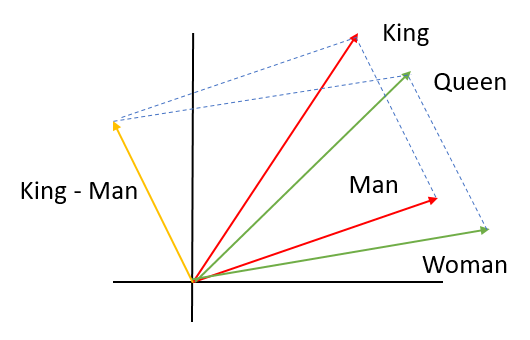
\includegraphics[scale = 0.5]{pictures/kingqueen}}

Famous vector addition example:
  
\centerline{King - Man + Woman $\approx$ Queen}

Note this picture is (very) \textit{schematic}. Embedding spaces are several hundred dimensional.

\end{frame}

\begin{frame}[fragile]{Bias}

\textcite{Caliskan.etal2017} replicate `implicit bias' using word embeddings
\begin{itemize}
  \item Experimental result: subjects pair two concepts they find similar faster than two concepts they find different. \parencite{Greenwald.etal1998} 
\end{itemize}

Operationalization in word embeddings: closer in space / more similar = shorter reaction time

\pause
\bigskip
Implicit bias is controversial (bias, less so) but we don't need to take a stand on the psychological theory
\begin{itemize}
  \item This is the usage!
\end{itemize}
\end{frame}

\begin{frame}[fragile]{Bias}

Their measure `WEAT' is computed in two steps (not how they describe it):
\begin{itemize}
  \item math average: cos(math words, male terms) - cos(math words to female terms)
  \item arts average: cos(math words, male terms) - cos(math words to female terms)
  \item math average - arts average
\end{itemize}
A `difference of differences'

\pause 

\medskip
\centerline{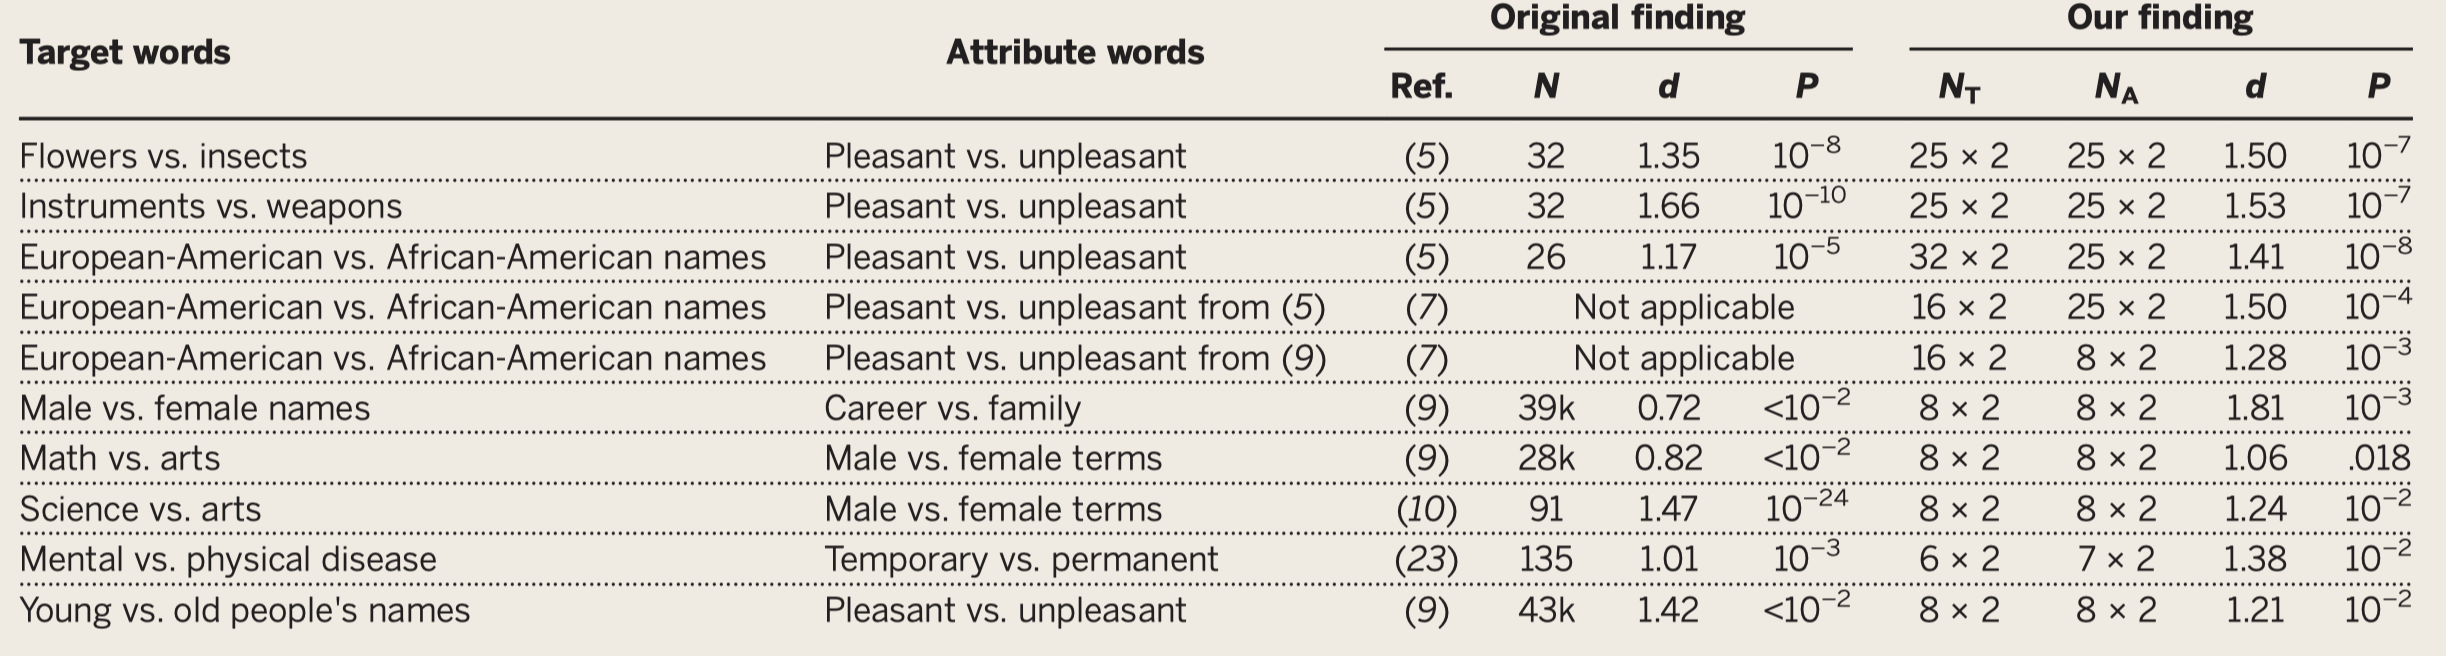
\includegraphics[scale = 0.3]{pictures/caliskan}}


\end{frame}


\begin{frame}[fragile]{Gender projection}

\centerline{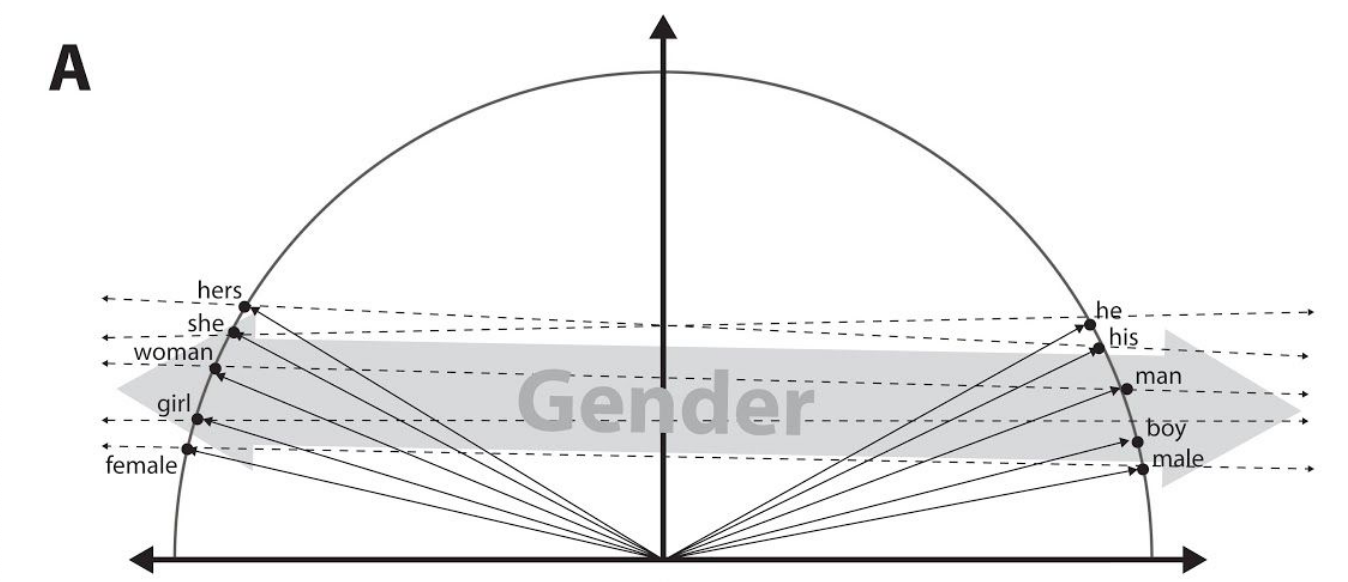
\includegraphics[scale = 0.5]{pictures/gender2}}

from \textcite{Kozlowski.etal2019}

\end{frame}
\begin{frame}[fragile]{Gender projection}

\centerline{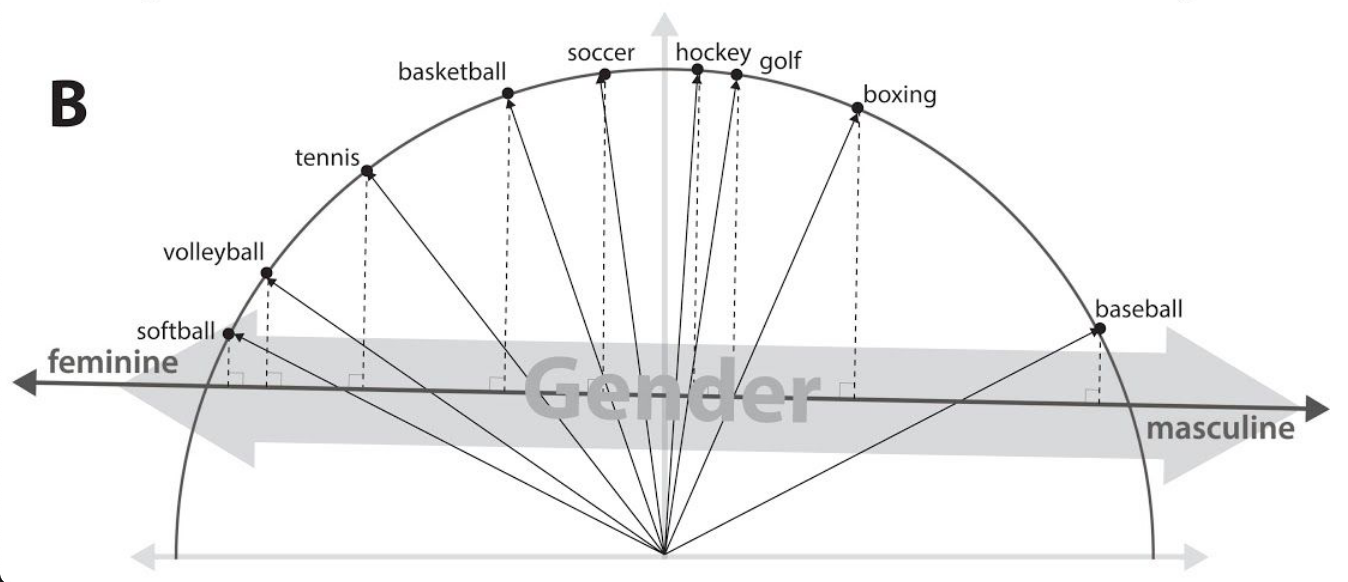
\includegraphics[scale = 0.5]{pictures/gender1}}

from \textcite{Kozlowski.etal2019}

\end{frame}


\begin{frame}[fragile]{Reflecting society}

\centerline{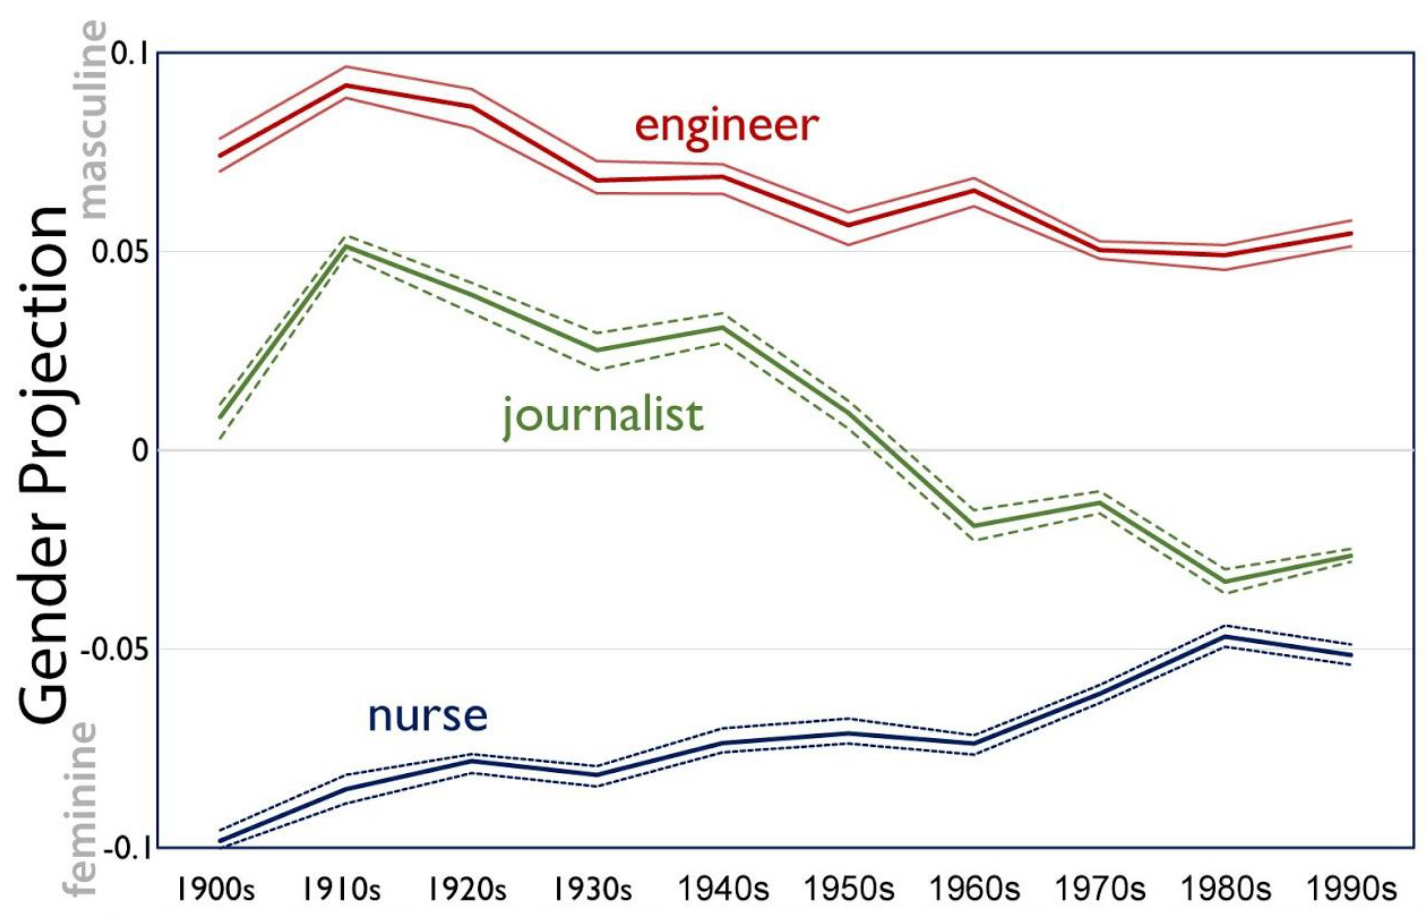
\includegraphics[scale = 0.4]{pictures/gender-proj}}

  from \textcite{Kozlowski.etal2019}
\end{frame}

\begin{frame}[fragile]{Reflecting society}

\centerline{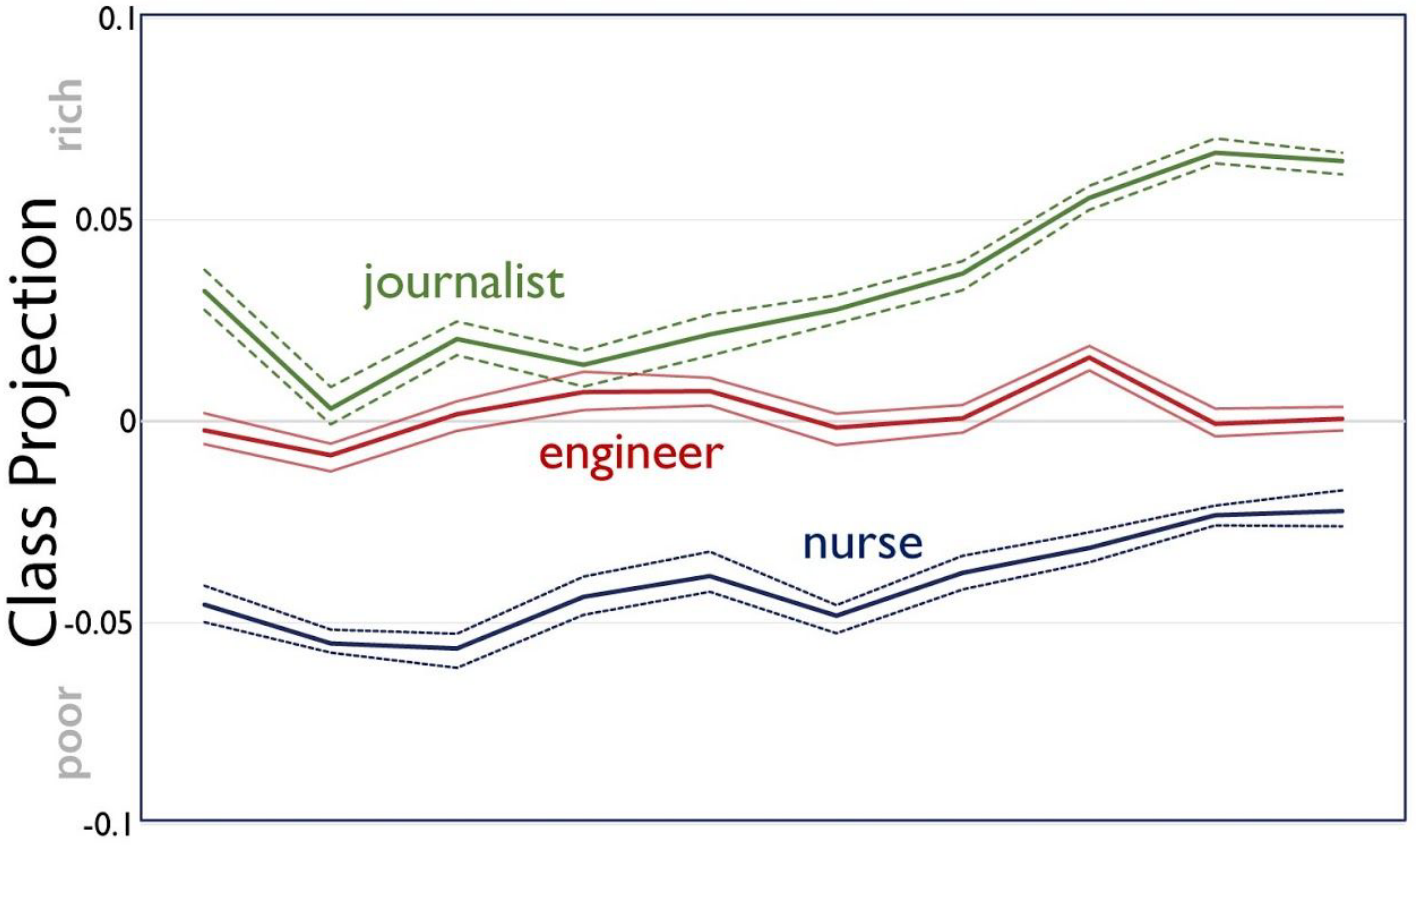
\includegraphics[scale = 0.4]{pictures/class-proj}}

  from \textcite{Kozlowski.etal2019}
\end{frame}

\begin{frame}{Reflecting society}

\centerline{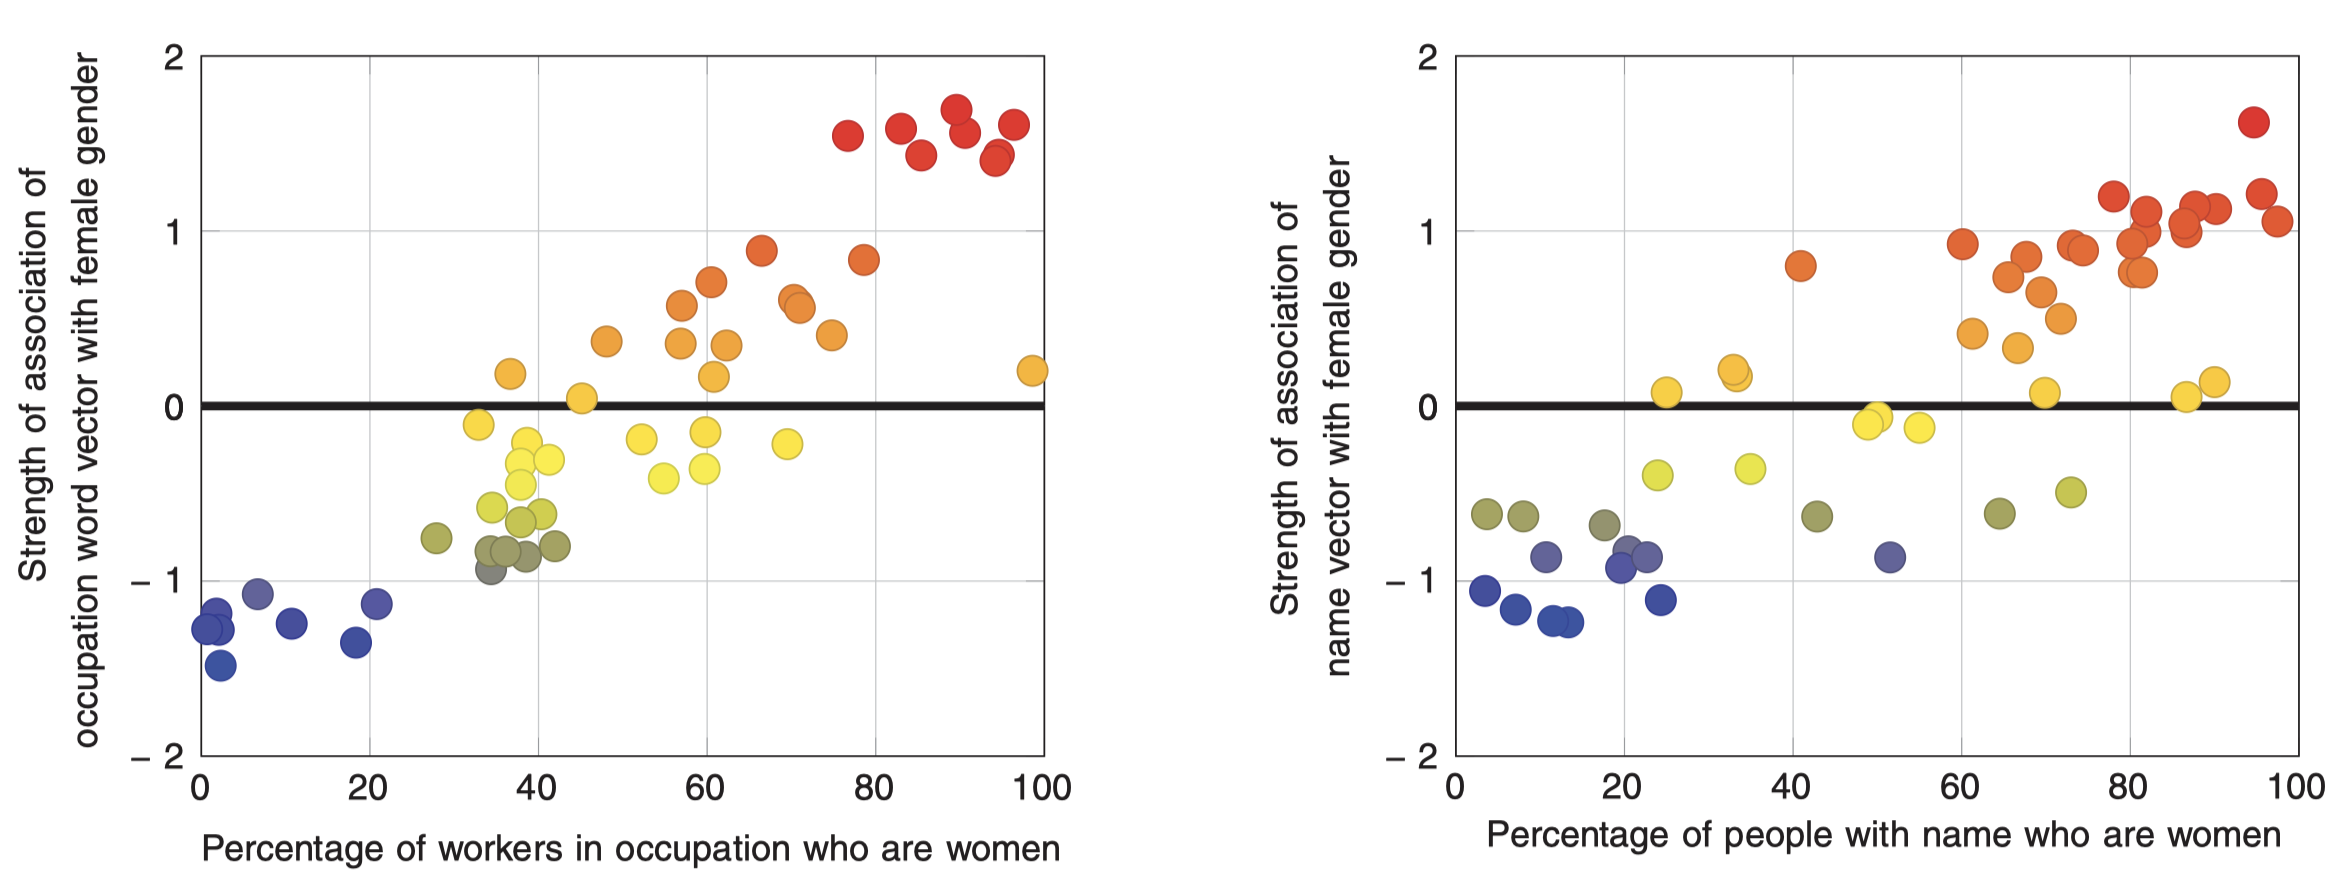
\includegraphics[scale = 0.3]{pictures/occupations-gender}}

from \textcite{Caliskan.etal2017}
\end{frame}

\begin{frame}{Reflecting society}

\centerline{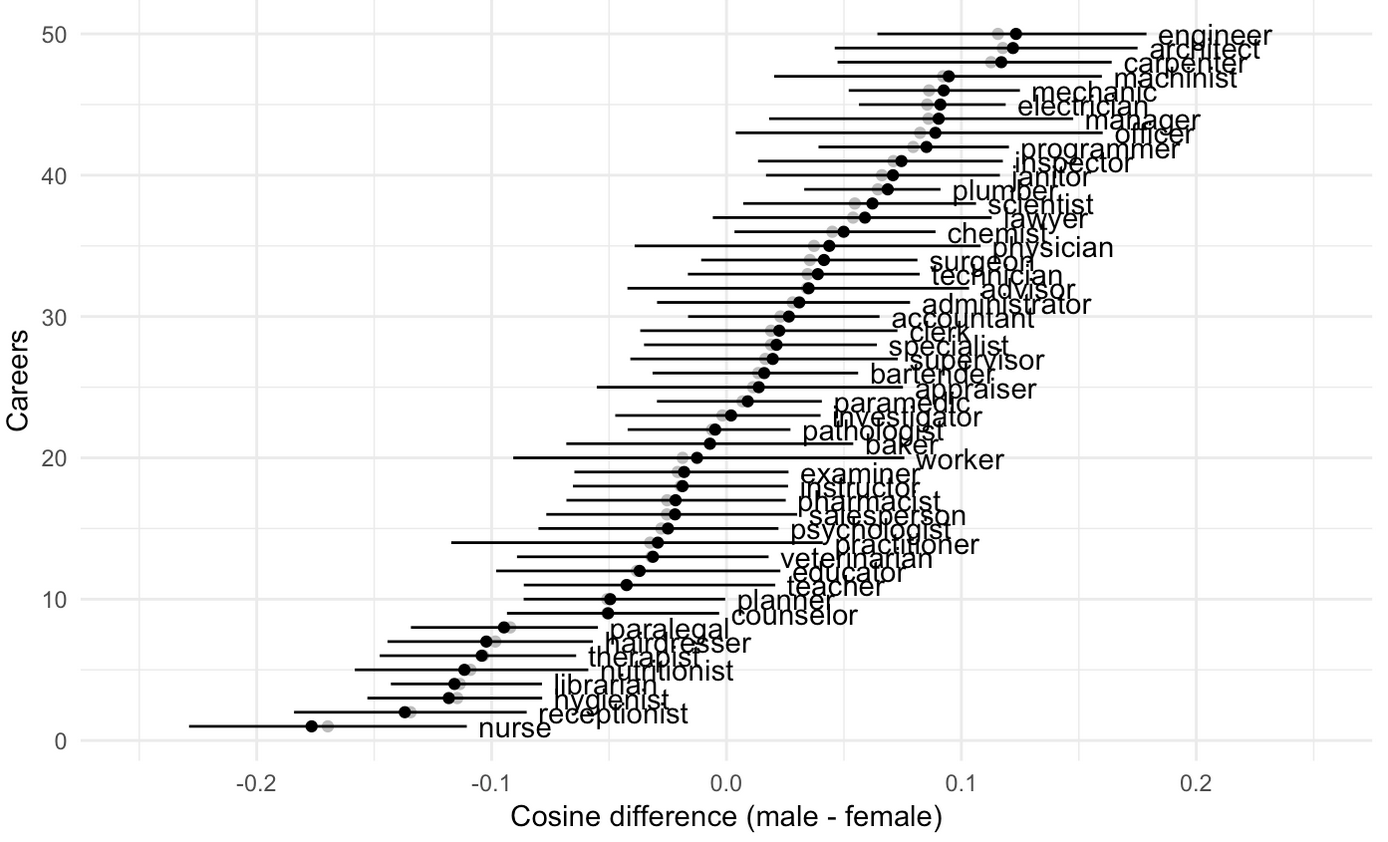
\includegraphics[scale = 0.5]{pictures/occupations-detail}}

redrawn from from \textcite{Caliskan.etal2017}

\end{frame}

\begin{frame}{Reflecting society}

\centerline{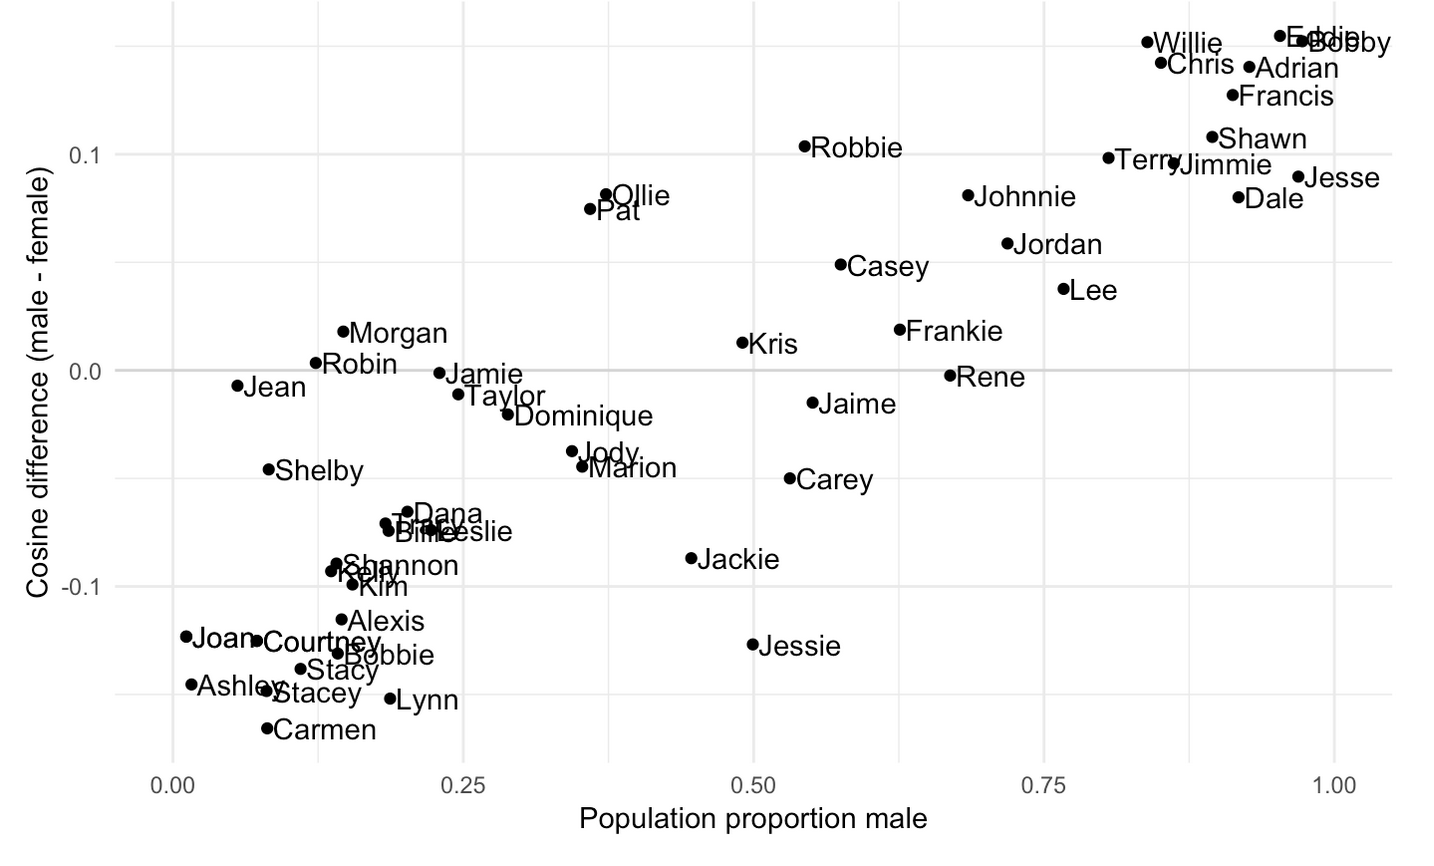
\includegraphics[scale = 0.4]{pictures/names-gender}}

redrawn from from \textcite{Caliskan.etal2017}

\end{frame}

\begin{frame}{Practicalities}

Word embeddings can be computationally intensive
\begin{itemize}
  \item for serious work: \textsf{gensim} (in python; Hurek 2020 \href{https://radimrehurek.com/gensim/}{[link]}) or \textsf{text2vec} (in R; Selivanov 2020 \href{http://text2vec.org}{[link]}) 
  \item for testing things out: LSA \href{https://quanteda.io/articles/pkgdown/examples/lsa.html}{[link]}
\end{itemize}
or you can just use some \textit{pre-computed} embeddings, e.g. from Google
\begin{itemize}
  \item \textsf{GloVe} makes available
\end{itemize}
\textcite{Rodriguez.Spirling2020} argue that this is usually just fine.
  
\end{frame}



\begin{frame}[allowframebreaks]
\frametitle{References}
\printbibliography	
\end{frame}


\end{document}